\documentclass{standalone}
\usepackage{tikz}
\begin{document}
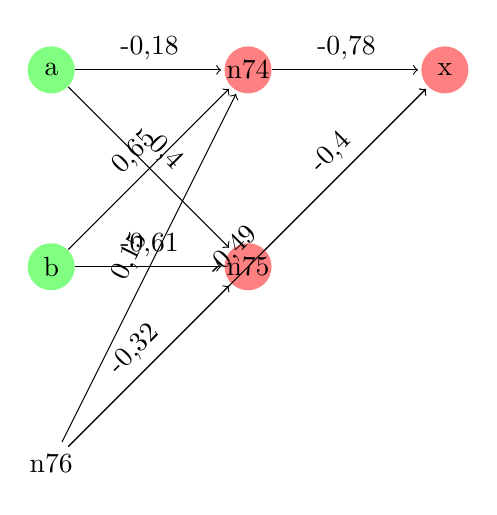
\begin{tikzpicture}[shorten >=1pt,->,draw=black!,node distance=2.5cm]
\tikzstyle{neuron}=[circle,fill=black!25,minimum size=17pt,inner sep=0pt]
\tikzstyle{constant}=[neuron, fill=white!50];
\tikzstyle{sigmoid}=[neuron, fill=red!50];
\tikzstyle{identity}=[neuron, fill=green!50];
\node [identity] (a) {a};
\node [identity,below of=a] (b) {b};
\node [constant,below of=b] (n76) {n76};
\node [sigmoid,right of=a] (n74) {n74};
\node [sigmoid,below of=n74] (n75) {n75};
\node [sigmoid,right of=n74] (x) {x};
\path[every node/.style={sloped,anchor=south,auto=false}]
(n74) edge node {-0,78} (x)
(n75) edge node {-0,4} (x)
(n76) edge node {-0,49} (x)
(n76) edge node {-0,32} (n75)
(n76) edge node {0,15} (n74)
(a) edge node {-0,18} (n74)
(a) edge node {0,4} (n75)
(b) edge node {-0,61} (n75)
(b) edge node {0,65} (n74)
;\end{tikzpicture}
\end{document}